\documentclass[9pt]{beamer}
\usetheme[titlepagelogo=minerva2,% Logo for the first page
						language=italian
                        ]{TorinoTh}
                        
\usepackage[beamer,customcolors]{hf-tikz}
\usepackage{verbatim}
\usepackage{algorithm}
\usepackage[noend]{algpseudocode}
\hfsetfillcolor{alerted text.fg!10}
\hfsetbordercolor{alerted text.fg}

\author{Marco Odore}
\rel{Prof. Giorgio Valentini}
\assistantsupervisor{Dr. Marco Notaro}
\title[Metodi di Ensemble Gerarchici]{Metodi di Ensemble Gerarchici per la Predizione Strutturata della Funzione delle Proteine}
\ateneo{Università Degli Studi Di Milano}
\date{10 Luglio 2018}

\begin{document}
\titlepageframe
\begin{tframe}{Il problema della predizione della funzione delle proteine}
  % 
  \begin{columns}
    %
    \begin{column}{.65\textwidth}
      \minipage[c][0.4\textheight][s]{\columnwidth}
	   \begin{itemize}	
      \onslide<1->
	  \item Identificare la funzione delle proteine attraverso le analisi di laboratorio è \highlightbf{costosa} e richiede \highlightbf{molto tempo}
	  \onslide<2->
	  \item Esistono centinaia di funzioni a cui poter associare un gene/proteina, anche contemporaneamente \highlightbf{(problema multiclasse e multietichetta)}
      \onslide<3->
	  \item Il quantitativo di dati genomici cresce molto rapidamente.
      \onslide<4->
	  \item La \highlightbf{classificazione manuale} delle proteine è quindi infattibile. È necessario quindi un approccio \highlightbf{automatico}.
	  \onslide<5->
	  \item A complicare ulteriormente il problema è il modo in cui sono \emph{relazionate} tra loro le funzioni delle proteine.
	  \end{itemize}
      \endminipage      
    \end{column}
    %
    \begin{column}{.35\textwidth}
      % for top aligned images use minipage
      \only<1-5>{
        \minipage[c][0.4\textheight][s]{\columnwidth}
        \onslide<1->    
        \only<1-5>{
          \begin{figure}
            \centering
            \includegraphics<1>[scale=0.15]{img/lab3.jpg} %         
            \includegraphics<2>[scale=0.3]{img/multilabel.png}%
            \includegraphics<3>[scale=0.16]{img/growth.jpg}
            \includegraphics<4>[scale=0.1]{img/machinelearning.png}
            \includegraphics<5>[scale=0.3]{img/relation.png}
        \end{figure}}
       \endminipage
      }   
      % for vertically centered images use parbox
    \end{column}
  \end{columns}
\end{tframe}

\begin{tframe}{Tassonomie per le funzioni delle proteine}
\begin{itemize}
\onslide<1->
\item Esistono infatti due tassonomie principali per l'organizzazione delle funzioni:
\begin{itemize}

\onslide<2->
\item \highlightbf{Gene Ontology} (GO):  che organizza le funzioni come un grafo diretto aciclico (DAG), varia per ogni specie, e possiede tre ontologie differenti (e quindi 3 DAG), e cioè \highlight{Biological Process} (BP), \highlight{Molecular Function} (MF) e \highlight{Cellular Component} (CC). 
\onslide<3->
\item \highlightbf{Functional Catalogue} (FunCat): che è organizzato invece come un albero, non varia in base alle specie, e descrive le funzioni in maniera più sintetica rispetto alla Gene Ontology.
\end{itemize}
\onslide<4->
\begin{figure}[h]
\center
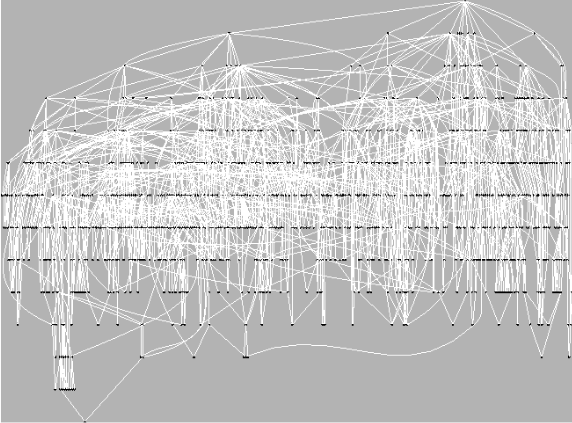
\includegraphics[scale=0.15]{./img/GO.png}
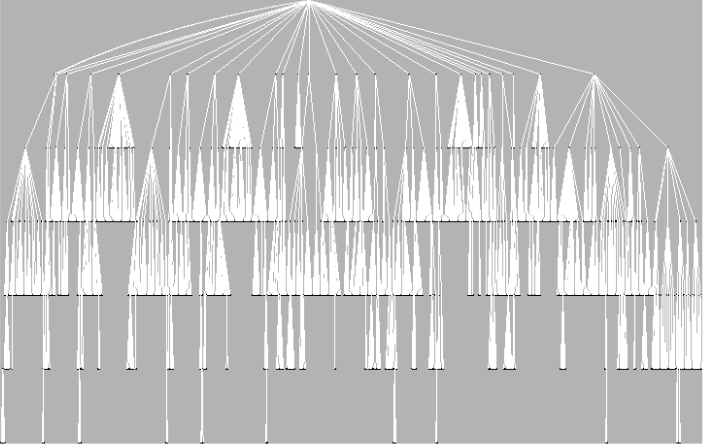
\includegraphics[scale=0.14]{./img/FunCat.png}
\label{DAGTREE}
\end{figure}
\onslide<5->
\item Data la granularità e specificità superiori della GO e il suo largo utilizzo nella comunità scientifica, all’interno della tesi ci si è soffermati sulla predizione delle sue funzioni.
\end{itemize}  
\end{tframe}

\begin{tframe}{La predizione della funzione delle proteine tramite metodi automatici}
I metodi più noti in letteratura per effettuare predizioni della funzione delle proteine in maniera automatica sono:

\begin{itemize}
\onslide<2->
\item I metodi basati sulla \highlightbf{comparazione di biosequenze}: si basano sull'idea che sequenze simili condividano funzioni simili.
\onslide<3->
\item I metodi \highlightbf{basati su reti}: sono metodi applicati a dati rappresentati sotto forma di reti, che si basano sugli algoritmi di propagazione delle etichette.
\onslide<4->
\item I metodi \highlightbf{Kernel per spazi di output strutturato}: sono metodi che sfruttano funzioni kernel congiunte per predire in spazi di output strutturato.
\onslide<5->
\item I metodi \highlightbf{Ensemble Gerarchici}: i metodi trattati in questa tesi.
\end{itemize}

\end{tframe}

\begin{tframe}{Metodi Ensemble Gerarchici 1/2}
I Metodi di Ensemble Gerarchici sono metodi caratterizzati da due step principali:

\begin{enumerate}
\onslide<2->
\item \highlightbf{Predizione flat} delle diverse classi dell’ontologia, generando diversi predittori \emph{indipendenti}.
\onslide<3->
\item \highlightbf{Combinazione e correzione gerarchica delle predizioni} sfruttando il DAG dei termini della GO.
\end{enumerate}
\onslide<4->
Il secondo step rappresenta la componente \emph{ensemble} del metodo. Tale step si rende necessario in quanto le predizioni flat non tengono in considerazione la struttura gerarchica dei DAG della GO, portando a risultati \emph{inconsistenti}.
\onslide<5->
\block{Consistenza \& True Path Rule}
Un insieme di predizioni $\hat{y} = <\hat{y}_1, \hat{y}_2, \dots, \hat{y}_{|N|}>$, dove $|N|$ è la cardinalità dei termini della gerarchia, è definito \emph{consistente}, se rispetta la \emph{True Path Rule}, e cioè:
\[
y\;\;\;consistente\;\; \leftrightarrow \forall i \in N, j \in par(i) \rightarrow y_j \geq y_i
\] 
Dove $par(i)$ indica l'insieme dei termini genitori del nodo $i$ nella gerarchia.
\endblock{}
\end{tframe}

\begin{tframe}{Metodi Ensemble Gerarchici (Esempio) 2/2}
\begin{center}
\includegraphics<1>[width=5cm]{img/1_1.png}
\includegraphics<2>[width=5cm]{img/2.png}
\includegraphics<3>[width=5cm]{img/3.png}
\includegraphics<4>[width=8.22cm]{img/4.png}
\end{center}

\end{tframe} 
\end{document}
